
\documentclass[12pt,fullpage]{exam}
\usepackage{color}
\usepackage{listings}
\usepackage{caption}
\usepackage{enumitem}
\usepackage{scrextend}
% \usepackage{amsmath,amssymb,xymtex,units}
\usepackage{amsmath}
\usepackage{minibox}
\usepackage[margin=0.8in]{geometry}
\usepackage{tikz}
% \usepackage{geometry}
% \geometry{legalpaper, landscape, margin=2in}
\usepackage[sans]{dsfont}
\usepackage{multicol,lipsum}
\usepackage{MnSymbol}
\usepackage[margin=1.5in]{geometry}    % For margin alignment
\usepackage[english]{babel}
\usepackage{minibox}
\usepackage[utf8]{inputenc}
\usepackage{algorithm}
\usepackage[noend]{algpseudocode}
\usepackage{mdframed}
\usepackage{lipsum}
\usepackage{amsthm}
\setlength{\columnsep}{2cm}
\setlength{\columnseprule}{1pt}
\newtheorem{theo}{Theorem}
\newenvironment{ftheo}
  {\begin{mdframed}\begin{theo}}
  {\end{theo}\end{mdframed}}
\newtheorem{theorem}{Theorem}[section]
\newtheorem{corollary}{Corollary}[theorem]
\newtheorem{lemma}[theorem]{Lemma}
\def\O{\mathcal{O}}
\newcommand{\pr}[1]{${#1}^{'}$}
\usepackage{listings}

\makeatletter
\lst@UserCommand\lstlistofcplusplus{\bgroup
    \let\contentsname\lstlistcplusplusname
    \let\lst@temp\@starttoc \def\@starttoc##1{\lst@temp{loc}}%
    \tableofcontents \egroup}
\lstnewenvironment{cplusplus}[1][]{%
  \renewcommand{\lstlistingname}{C++ Code}%
  \xpatchcmd{\lst@MakeCaption}{}{}{}{}%
  \lstset{language=bash,#1,frame=none}}
  {}
\lstset{
  basicstyle=\ttfamily\footnotesize,,
  xleftmargin=3em,
  frame=leftline,
  framerule=1pt,
  framexleftmargin=1pt,
  mathescape,  
  literate={->}{$\rightarrow$}{2}
           {α}{$\alpha$}{1}
           {δ}{$\delta$}{1}
}
% \DeclareCaptionLabelFormat{algocaption}{Algorithm} % defines a new caption label as Algorithm x.y
\usepackage{graphicx}
\graphicspath{ {.} }

\usepackage{mathtools}
\DeclarePairedDelimiter{\floor}{\lfloor}{\rfloor}
\printanswers
 \input amssym.tex
%%%%%%
\begin{document}

\title{ASSIGNMENT 2}%replace X with the appropriate number
\author{KESHAV BANSAL(170335)\\~\\%replace with your name
CS335}
\date{}
\maketitle
\begin{questions}

\section*{Question}
\question \textbf{For the following grammar, design a predictive parser and show the predictive parsing table. Remove
left-recursion (if any), left-factor your grammar.\\
$S$ $\rightarrow$ $(L)$ $|$ $a$\\
$L$ $\rightarrow$ $L,S$ $|$ $LS$ $|$ $b$}


\textbf{Solution}\\

\textbf{Grammar after removing left recursion}:\\
\indent{
$S$ $\rightarrow$ $(L)$ $|$ $a$\\
$L$ $\rightarrow$ $bX$ \\
$X$ $\rightarrow$ $,SX$ $|$ $SX$ $|$ $\epsilon$\\
}
\textbf{First and follow set computation} : 

First($L$) = $\{$  $b$   $\}$

First($S$) = $\{$ $($ , $a$  $\}$

First($X$) = $\{$ `,' , $($ , $a$ , $\epsilon$   $\}$

Follow($L$) = $\{$  $)$   $\}$

Follow($S$) = $\{$ `,' , $($ , $a$ , $\$$, )  $\}$

Follow($X$) = $\{$ ) $\}$\\~\\
\fbox{Note: `,' is used to denote the terminal comma(,) in the grammar}

\textbf{Predictive parsing table} :

\begin{table}[H]
\centering
\begin{tabular}{|c|l|l|l|l|l|l|}
\hline
\textbf{Nonterminal} &
  \multicolumn{1}{c|}{\textbf{(}} &
  \multicolumn{1}{c|}{\textbf{)}} &
  \multicolumn{1}{c|}{\textbf{`,'}} &
  \multicolumn{1}{c|}{\textbf{a}} &
  \multicolumn{1}{c|}{\textbf{b}} &
  \multicolumn{1}{c|}{\textbf{\$}} \\ \hline
\textbf{S} & $S$ $\rightarrow$ $(L)$ &                              &                         & $S$ $\rightarrow$ $a$  &                        &  \\ \hline
\textbf{L} &                         &                              &                         &                        & $L$ $\rightarrow$ $bX$ &  \\ \hline
\textbf{X} & $X$ $\rightarrow$ $SX$  & $X$ $\rightarrow$ $\epsilon$ & $X$ $\rightarrow$ $,SX$ & $X$ $\rightarrow$ $SX$ &                        &  \\ \hline
\end{tabular}

\end{table}
\section*{Question}
\question \textbf{Show that the given grammar is LALR(1) but not SLR(1).}

\textbf{Adding a dummy start state $S^{'}$ we get the following rules :}

\begin{lstlisting}
1) S$^{'}$ -> S
2) S -> Lp
3) S -> qLr
4) S -> sr
5) S -> qsp
6) L -> s
\end{lstlisting}
\textbf{Canonical states :}\\

\begin{multicols}{2}
$I_0$ $=$ 
\begin{lstlisting}
 S$^{'}$ -> .S
 S -> .Lp
 S -> .qLr
 S -> .sr
 S -> .qsp
 L -> .s
\end{lstlisting}

$I_1$ $=$ goto($I_0$,$S$) =
\begin{lstlisting}
 S$^{'}$ -> S.
\end{lstlisting}
$I_2$ $=$ goto($I_0$,$L$) =
\begin{lstlisting}
S -> L.p
\end{lstlisting}

$I_3$ $=$ goto($I_0$,$q$) =
\begin{lstlisting}
S->q.Lr
S->q.sp
L->.s
\end{lstlisting}
$I_4$ $=$ goto($I_0$,$s$) =
\begin{lstlisting}
S->s.r
L->s.
\end{lstlisting}

$I_5$ $=$ goto($I_2$,$p$) =
\begin{lstlisting}
S->Lp.

\end{lstlisting}
\columnbreak
$I_6$ $=$ goto($I_3$,$L$) =
\begin{lstlisting}
S->qL.r
\end{lstlisting}

$I_7$ $=$ goto($I_3$,$s$) =
\begin{lstlisting}
S->qs.p
L->s.
\end{lstlisting}
$I_8$ $=$ goto($I_4$,$r$) =
\begin{lstlisting}
S->sr.
\end{lstlisting}

$I_9$ $=$ goto($I_6$,$r$) =
\begin{lstlisting}
S->qLr.
\end{lstlisting}

$I_{10}$ $=$ goto($I_7$,$p$) =
\begin{lstlisting}
S->qsp.
\end{lstlisting}
\end{multicols}

{\minibox[frame]{
FOLLOW($S^{'}$) = \{$\$$\} \\

FOLLOW($S$) = \{$\$$\}\\

FOLLOW($L$) = \{$p,r$\}\\
}
}
\\~\\
% Please add the following required packages to your document preamble:
% \usepackage{multirow}
\begin{table}[H]
\centering
\begin{tabular}{|l|l|l|l|l|l|l|l|l|}
\hline
\multirow{\textbf{STATE}} & \multicolumn{5}{l|}{\textbf{ACTION}}   & \multicolumn{3}{l|}{\textbf{GOTO}} \\ \cline{2-9} 
                                & p                                                   & q  & r                                               & s  & \$     & S'         & S         & L         \\ \hline
\textbf{0}                      &                                                     & s3 &                                                 & s4 &        &            & 1         & 2         \\ \hline
\textbf{1}                      &                                                     &    &                                                 &    & accept &            &           &           \\ \hline
\textbf{2}                      & s5                                                 &    &                                                 &    &        &            &           &           \\ \hline
\textbf{3}                      &                                                     &    &                                                 & s7 &        &            &           & 6         \\ \hline
\textbf{4}                      & r6                                                  &    & \begin{tabular}[c]{@{}l@{}}r6\\ s8\end{tabular} &    &        &            &           &           \\ \hline
\textbf{5}                      &                                                     &    &                                                 &    & r2     &            &           &           \\ \hline
\textbf{6}                      &                                                     &    & s9                                              &    &        &            &           &           \\ \hline
\textbf{7}                      & \begin{tabular}[c]{@{}l@{}}r6\\ \\ s10\end{tabular} &    & r6                                              &    &        &            &           &           \\ \hline
\textbf{8}                      &                                                     &    &                                                 &    & r4     &            &           &           \\ \hline
\textbf{9}                      &                                                     &    &                                                 &    & r3     &            &           &           \\ \hline
\textbf{10}                     &                                                     &    &                                                 &    & r5     &            &           &           \\ \hline
\end{tabular}
\caption{Parse table for SLR(1)}
\end{table}

\textbf{Since there are 2 shift reduce conficts, the grammar is SLR(1) ambiguous.}

\textbf{Canonical states for LALR(1):}

\begin{multicols}{2}
$I_0$ $=$ 
\begin{lstlisting}
 S$^{'}$ -> .S , $\$$
 S -> .Lp , $\$$
 S -> .qLr , $\$$
 S -> .sr , $\$$
 S -> .qsp , $\$$
 L -> .s , $p$
\end{lstlisting}

$I_1$ $=$ goto($I_0$,$S$) =
\begin{lstlisting}
 S$^{'}$ -> S. , $\$$
\end{lstlisting}
$I_2$ $=$ goto($I_0$,$L$) =
\begin{lstlisting}
S -> L.p , $\$$
\end{lstlisting}

$I_3$ $=$ goto($I_0$,$q$) =
\begin{lstlisting}
S->q.Lr , $\$$
S->q.sp , $\$$
L->.s , $r$
\end{lstlisting}
$I_4$ $=$ goto($I_0$,$s$) =
\begin{lstlisting}
S->s.r , $\$$
L->s. , $p$
\end{lstlisting}

$I_5$ $=$ goto($I_2$,$p$) =
\begin{lstlisting}
S->Lp. , $\$$

\end{lstlisting}
\columnbreak
$I_6$ $=$ goto($I_3$,$L$) =
\begin{lstlisting}
S->qL.r , $\$$

\end{lstlisting}

$I_7$ $=$ goto($I_3$,$s$) =
\begin{lstlisting}
S->qs.p , $\$$
L->s. , $r$
\end{lstlisting}
$I_8$ $=$ goto($I_4$,$r$) =
\begin{lstlisting}
S->sr. , $\$$
\end{lstlisting}

$I_9$ $=$ goto($I_6$,$r$) =
\begin{lstlisting}
S->qLr. , $\$$
\end{lstlisting}

$I_{10}$ $=$ goto($I_7$,$p$) =
\begin{lstlisting}
S->qsp. , $\$$
\end{lstlisting}
\end{multicols}

\begin{figure}[H]


\begin{center}
\centering



\tikzset{every picture/.style={line width=0.75pt}} %set default line width to 0.75pt        

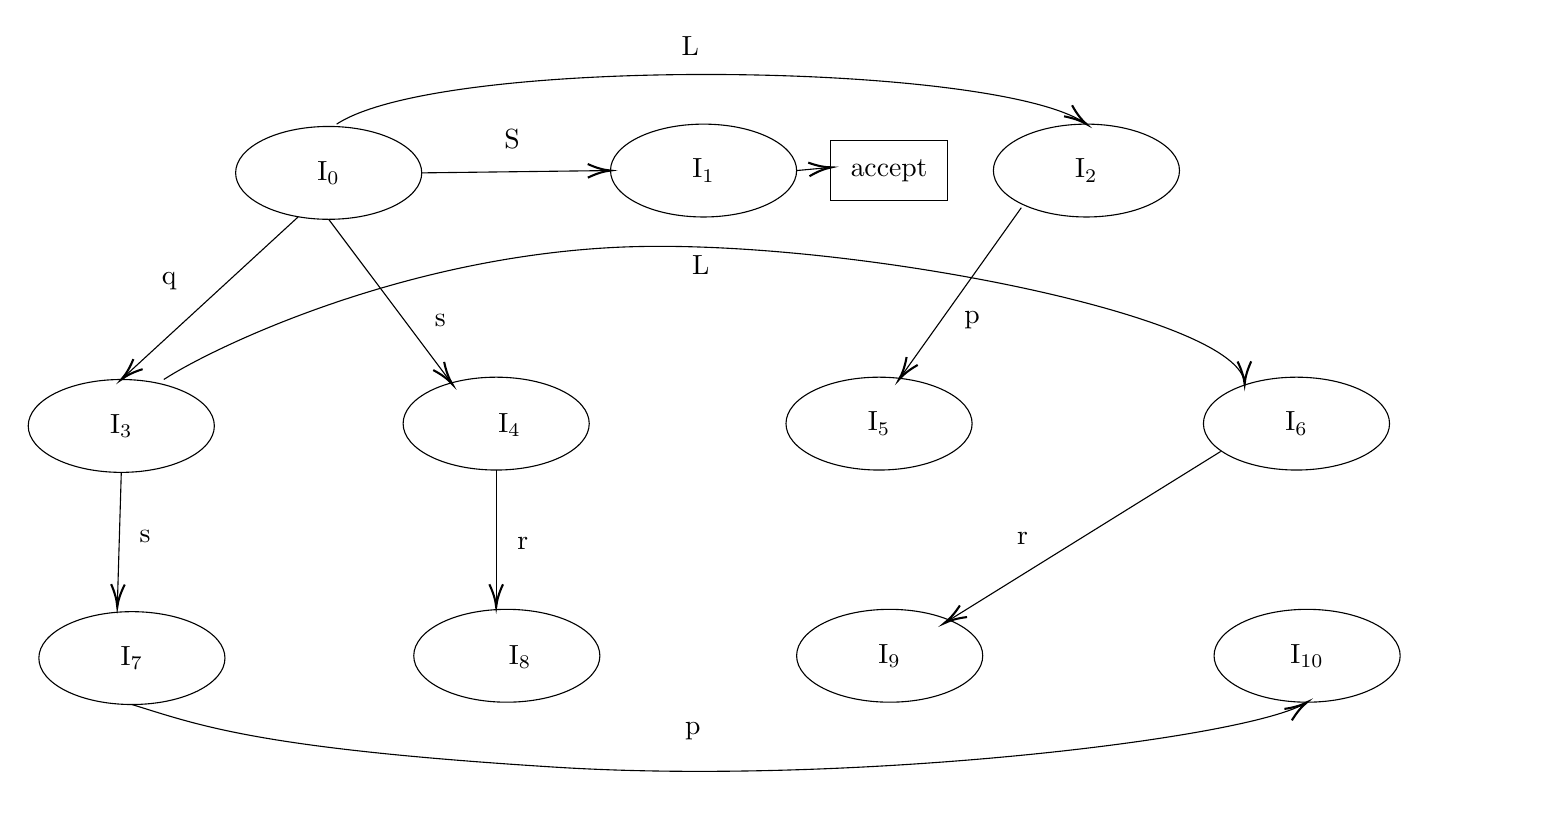
\begin{tikzpicture}[x=0.75pt,y=0.75pt,yscale=-1,xscale=1]
%uncomment if require: \path (0,360); %set diagram left start at 0, and has height of 360

%Shape: Ellipse [id:dp2946130813265617] 
\draw   (181.12,192.46) .. controls (181.12,180.1) and (201.2,170.09) .. (225.96,170.09) .. controls (250.72,170.09) and (270.79,180.1) .. (270.79,192.46) .. controls (270.79,204.81) and (250.72,214.83) .. (225.96,214.83) .. controls (201.2,214.83) and (181.12,204.81) .. (181.12,192.46) -- cycle ;
%Shape: Ellipse [id:dp4654909418726765] 
\draw   (0.5,193.58) .. controls (0.5,181.22) and (20.57,171.21) .. (45.34,171.21) .. controls (70.1,171.21) and (90.17,181.22) .. (90.17,193.58) .. controls (90.17,205.93) and (70.1,215.95) .. (45.34,215.95) .. controls (20.57,215.95) and (0.5,205.93) .. (0.5,193.58) -- cycle ;
%Shape: Ellipse [id:dp26335781773898925] 
\draw   (365.59,192.46) .. controls (365.59,180.1) and (385.66,170.09) .. (410.42,170.09) .. controls (435.18,170.09) and (455.26,180.1) .. (455.26,192.46) .. controls (455.26,204.81) and (435.18,214.83) .. (410.42,214.83) .. controls (385.66,214.83) and (365.59,204.81) .. (365.59,192.46) -- cycle ;
%Shape: Ellipse [id:dp7257142726038222] 
\draw   (566.71,192.46) .. controls (566.71,180.1) and (586.78,170.09) .. (611.54,170.09) .. controls (636.3,170.09) and (656.38,180.1) .. (656.38,192.46) .. controls (656.38,204.81) and (636.3,214.83) .. (611.54,214.83) .. controls (586.78,214.83) and (566.71,204.81) .. (566.71,192.46) -- cycle ;
%Shape: Ellipse [id:dp3539845497539733] 
\draw   (281.04,70.54) .. controls (281.04,58.19) and (301.11,48.17) .. (325.88,48.17) .. controls (350.64,48.17) and (370.71,58.19) .. (370.71,70.54) .. controls (370.71,82.9) and (350.64,92.91) .. (325.88,92.91) .. controls (301.11,92.91) and (281.04,82.9) .. (281.04,70.54) -- cycle ;
%Shape: Ellipse [id:dp476543140903408] 
\draw   (100.42,71.66) .. controls (100.42,59.3) and (120.49,49.29) .. (145.25,49.29) .. controls (170.02,49.29) and (190.09,59.3) .. (190.09,71.66) .. controls (190.09,84.01) and (170.02,94.03) .. (145.25,94.03) .. controls (120.49,94.03) and (100.42,84.01) .. (100.42,71.66) -- cycle ;
%Shape: Ellipse [id:dp5726803177881032] 
\draw   (465.51,70.54) .. controls (465.51,58.19) and (485.58,48.17) .. (510.34,48.17) .. controls (535.1,48.17) and (555.18,58.19) .. (555.18,70.54) .. controls (555.18,82.9) and (535.1,92.91) .. (510.34,92.91) .. controls (485.58,92.91) and (465.51,82.9) .. (465.51,70.54) -- cycle ;
%Shape: Ellipse [id:dp963814868521595] 
\draw   (186.25,304.31) .. controls (186.25,291.95) and (206.32,281.94) .. (231.08,281.94) .. controls (255.84,281.94) and (275.92,291.95) .. (275.92,304.31) .. controls (275.92,316.66) and (255.84,326.68) .. (231.08,326.68) .. controls (206.32,326.68) and (186.25,316.66) .. (186.25,304.31) -- cycle ;
%Shape: Ellipse [id:dp5971384034374021] 
\draw   (5.62,305.43) .. controls (5.62,293.07) and (25.7,283.06) .. (50.46,283.06) .. controls (75.22,283.06) and (95.29,293.07) .. (95.29,305.43) .. controls (95.29,317.78) and (75.22,327.8) .. (50.46,327.8) .. controls (25.7,327.8) and (5.62,317.78) .. (5.62,305.43) -- cycle ;
%Shape: Ellipse [id:dp8955562762594678] 
\draw   (370.71,304.31) .. controls (370.71,291.95) and (390.78,281.94) .. (415.55,281.94) .. controls (440.31,281.94) and (460.38,291.95) .. (460.38,304.31) .. controls (460.38,316.66) and (440.31,326.68) .. (415.55,326.68) .. controls (390.78,326.68) and (370.71,316.66) .. (370.71,304.31) -- cycle ;
%Shape: Ellipse [id:dp0440823393108114] 
\draw   (571.83,304.31) .. controls (571.83,291.95) and (591.9,281.94) .. (616.66,281.94) .. controls (641.43,281.94) and (661.5,291.95) .. (661.5,304.31) .. controls (661.5,316.66) and (641.43,326.68) .. (616.66,326.68) .. controls (591.9,326.68) and (571.83,316.66) .. (571.83,304.31) -- cycle ;
%Straight Lines [id:da22129259569374904] 
\draw    (190.09,71.66) -- (279.04,70.56) ;
\draw [shift={(281.04,70.54)}, rotate = 539.3] [color={rgb, 255:red, 0; green, 0; blue, 0 }  ][line width=0.75]    (10.93,-3.29) .. controls (6.95,-1.4) and (3.31,-0.3) .. (0,0) .. controls (3.31,0.3) and (6.95,1.4) .. (10.93,3.29)   ;
%Curve Lines [id:da5970897279705547] 
\draw    (149.1,48.17) .. controls (199.82,14.95) and (463.36,17.91) .. (509.02,47.27) ;
\draw [shift={(510.34,48.17)}, rotate = 215.96] [color={rgb, 255:red, 0; green, 0; blue, 0 }  ][line width=0.75]    (10.93,-3.29) .. controls (6.95,-1.4) and (3.31,-0.3) .. (0,0) .. controls (3.31,0.3) and (6.95,1.4) .. (10.93,3.29)   ;
%Straight Lines [id:da10101803840461487] 
\draw    (130.52,92.91) -- (46.81,169.85) ;
\draw [shift={(45.34,171.21)}, rotate = 317.40999999999997] [color={rgb, 255:red, 0; green, 0; blue, 0 }  ][line width=0.75]    (10.93,-3.29) .. controls (6.95,-1.4) and (3.31,-0.3) .. (0,0) .. controls (3.31,0.3) and (6.95,1.4) .. (10.93,3.29)   ;
%Straight Lines [id:da9960793852692429] 
\draw    (145.25,94.03) -- (203.62,171.84) ;
\draw [shift={(204.82,173.44)}, rotate = 233.13] [color={rgb, 255:red, 0; green, 0; blue, 0 }  ][line width=0.75]    (10.93,-3.29) .. controls (6.95,-1.4) and (3.31,-0.3) .. (0,0) .. controls (3.31,0.3) and (6.95,1.4) .. (10.93,3.29)   ;
%Straight Lines [id:da6759182560123711] 
\draw    (478.96,88.44) -- (421.19,169.58) ;
\draw [shift={(420.03,171.21)}, rotate = 305.45] [color={rgb, 255:red, 0; green, 0; blue, 0 }  ][line width=0.75]    (10.93,-3.29) .. controls (6.95,-1.4) and (3.31,-0.3) .. (0,0) .. controls (3.31,0.3) and (6.95,1.4) .. (10.93,3.29)   ;
%Curve Lines [id:da19794814351808632] 
\draw    (65.83,171.21) .. controls (87.97,156.71) and (178.94,112.18) .. (285.52,107.45) .. controls (390.51,102.79) and (580.39,139.28) .. (586.41,171.95) ;
\draw [shift={(586.56,173.44)}, rotate = 269.37] [color={rgb, 255:red, 0; green, 0; blue, 0 }  ][line width=0.75]    (10.93,-3.29) .. controls (6.95,-1.4) and (3.31,-0.3) .. (0,0) .. controls (3.31,0.3) and (6.95,1.4) .. (10.93,3.29)   ;
%Straight Lines [id:da10011357349324967] 
\draw    (45.34,215.95) -- (43.47,278.82) ;
\draw [shift={(43.41,280.82)}, rotate = 271.7] [color={rgb, 255:red, 0; green, 0; blue, 0 }  ][line width=0.75]    (10.93,-3.29) .. controls (6.95,-1.4) and (3.31,-0.3) .. (0,0) .. controls (3.31,0.3) and (6.95,1.4) .. (10.93,3.29)   ;
%Straight Lines [id:da5113366441424965] 
\draw    (225.96,214.83) -- (225.96,278.82) ;
\draw [shift={(225.96,280.82)}, rotate = 270] [color={rgb, 255:red, 0; green, 0; blue, 0 }  ][line width=0.75]    (10.93,-3.29) .. controls (6.95,-1.4) and (3.31,-0.3) .. (0,0) .. controls (3.31,0.3) and (6.95,1.4) .. (10.93,3.29)   ;
%Straight Lines [id:da4821824879472565] 
\draw    (575.03,205.88) -- (443.51,287.59) ;
\draw [shift={(441.81,288.65)}, rotate = 328.15] [color={rgb, 255:red, 0; green, 0; blue, 0 }  ][line width=0.75]    (10.93,-3.29) .. controls (6.95,-1.4) and (3.31,-0.3) .. (0,0) .. controls (3.31,0.3) and (6.95,1.4) .. (10.93,3.29)   ;
%Curve Lines [id:da7418686148637745] 
\draw    (50.46,327.8) .. controls (83.13,337.86) and (111.31,349.05) .. (254.78,358) .. controls (396.1,366.81) and (584.4,344.72) .. (615.36,327.46) ;
\draw [shift={(616.66,326.68)}, rotate = 506.78] [color={rgb, 255:red, 0; green, 0; blue, 0 }  ][line width=0.75]    (10.93,-3.29) .. controls (6.95,-1.4) and (3.31,-0.3) .. (0,0) .. controls (3.31,0.3) and (6.95,1.4) .. (10.93,3.29)   ;
%Shape: Rectangle [id:dp5650014411972386] 
\draw   (387,56) -- (443.5,56) -- (443.5,85) -- (387,85) -- cycle ;
%Straight Lines [id:da7471396021636194] 
\draw    (370.71,70.54) -- (385.51,69.18) ;
\draw [shift={(387.5,69)}, rotate = 534.76] [color={rgb, 255:red, 0; green, 0; blue, 0 }  ][line width=0.75]    (10.93,-3.29) .. controls (6.95,-1.4) and (3.31,-0.3) .. (0,0) .. controls (3.31,0.3) and (6.95,1.4) .. (10.93,3.29)   ;

% Text Node
\draw (721,21) node    {};
% Text Node
\draw (701,71) node    {};
% Text Node
\draw (722,251) node    {};
% Text Node
\draw (702,301) node    {};
% Text Node
\draw (145.25,71.66) node   [align=left] {I\textsubscript{0}};
% Text Node
\draw (510.34,70.54) node   [align=left] {I\textsubscript{2}};
% Text Node
\draw (325.88,70.54) node   [align=left] {I\textsubscript{1}};
% Text Node
\draw (410.42,192.46) node   [align=left] {I\textsubscript{5}};
% Text Node
\draw (232.36,193.02) node   [align=left] {I\textsubscript{4}};
% Text Node
\draw (45.34,193.58) node   [align=left] {I\textsubscript{3}};
% Text Node
\draw (611.54,192.46) node   [align=left] {I\textsubscript{6}};
% Text Node
\draw (415.55,304.31) node   [align=left] {I\textsubscript{9}};
% Text Node
\draw (237.49,304.87) node   [align=left] {I\textsubscript{8}};
% Text Node
\draw (50.46,305.43) node   [align=left] {I\textsubscript{7}};
% Text Node
\draw (616.66,304.31) node   [align=left] {I\textsubscript{10}};
% Text Node
\draw (233.64,55.44) node   [align=left] {S};
% Text Node
\draw (319.47,10.7) node   [align=left] {L};
% Text Node
\draw (324.59,115.84) node   [align=left] {L};
% Text Node
\draw (199.06,142.68) node   [align=left] {s};
% Text Node
\draw (455.26,142.68) node   [align=left] {p};
% Text Node
\draw (56.86,246.7) node   [align=left] {s};
% Text Node
\draw (238.77,250.06) node   [align=left] {r};
% Text Node
\draw (479.6,247.82) node   [align=left] {r};
% Text Node
\draw (320.75,340.66) node   [align=left] {p};
% Text Node
\draw (68.39,123.67) node   [align=left] {q};
% Text Node
\draw (415.25,70.5) node   [align=left] {accept};


\end{tikzpicture}


\end{center}
    \caption{State diagram for SLR and LALR parser}
    \label{fig:my_label}
\end{figure}
\begin{table}[H]
\centering
\begin{tabular}{|l|l|l|l|l|l|l|l|l|}
\hline
\multirow{\textbf{STATE}} & \multicolumn{5}{l|}{\textbf{ACTION}} & \multicolumn{3}{l|}{\textbf{GOTO}} \\ \cline{2-9} 
                                & p     & q    & r    & s    & \$      & S'         & S         & L         \\ \hline
\textbf{0}                      &       & s3   &      & s4   &         &            & 1         & 2         \\ \hline
\textbf{1}                      &       &      &      &      & accept  &            &           &           \\ \hline
\textbf{2}                      & s5    &      &      &      &         &            &           &           \\ \hline
\textbf{3}                      &       &      &      & s7   &         &            &           & 6         \\ \hline
\textbf{4}                      & r6    &      & s8   &      &         &            &           &           \\ \hline
\textbf{5}                      &       &      &      &      & r2      &            &           &           \\ \hline
\textbf{6}                      &       &      & s9   &      &         &            &           &           \\ \hline
\textbf{7}                      & s10   &      & r6   &      &         &            &           &           \\ \hline
\textbf{8}                      &       &      &      &      & r4      &            &           &           \\ \hline
\textbf{9}                      &       &      &      &      & r3      &            &           &           \\ \hline
\textbf{10}                     &       &      &      &      & r5      &            &           &           \\ \hline
\end{tabular}
\caption{Parse table for LALR(1)}
\end{table}

\textbf{Since each cell contains atmost one action, the grammar is LALR(1) }
\section*{Question}
\question \textbf{Construct an SLR parsing table for the given grammar. Resolve the parsing action conflicts in such a way that regular expressions will be parsed
normally.}

\textbf{Adding a dummy start state $S$ we get the following rules :}
\begin{lstlisting}
1) S -> R
2) R -> R | R
3) R -> RR
4) R -> R$^\ast$
5) R -> (R)
6) R -> a
7) R -> b
\end{lstlisting}
\textbf{Canonical states}\\
\begin{multicols}{2}
$I_0$ $=$ 
\begin{lstlisting}
 S -> .R
 R -> .R | R
 R -> .RR
 R -> .R$^\ast$
 R -> .(R)
 R -> .a
 R -> .b

\end{lstlisting}

$I_1$ $=$ goto($I_0$,$R$) =
\begin{lstlisting}
 S -> R.
 R -> R. | R
 R -> R.R
 R -> R.$^\ast$
 R -> .R | R
 R -> .RR
 R -> .R$^\ast$
 R -> .(R)
 R -> .a
 R -> .b

\end{lstlisting}
$I_2$ $=$ goto($I_0$,$($) =
\begin{lstlisting}
R->(.R)
R->.R|R
R->.RR
R->.R$^\ast$
R->.(R)
R->.a
R->.b

\end{lstlisting}

$I_3$ $=$ goto($I_0$,$a$) =
\begin{lstlisting}
R->a.


\end{lstlisting}
$I_4$ $=$ goto($I_0$,$b$) =
\begin{lstlisting}
R->b.
\end{lstlisting}

$I_5$ $=$ goto($I_1$,$|$) =
\begin{lstlisting}
R->R|.R
R->.R|R
R->.RR
R->.R$^\ast$
R->.(R)
R->.a
R->.b

\end{lstlisting}
$I_6$ $=$ goto($I_1$,$*$) =
\begin{lstlisting}
R->R$^\ast$.

\end{lstlisting}

$I_7$ $=$ goto($I_1$,$R$) =
\begin{lstlisting}
R->RR.
R->R.|R
R->R.R
R->R.$^*$
R->.R|R
R->.RR
R->.R$^*$
R->.(R)
R->.a
R->.b

\end{lstlisting}
$I_8$ $=$ goto($I_2$,$R$) =
\begin{lstlisting}
R->(R.)
R->R.|R
R->R.R
R->R.$^*$
R->.R|R
R->.RR
R->.(R)
R->.a
R->.b

\end{lstlisting}

$I_9$ $=$ goto($I_5$,$R$) =
\begin{lstlisting}
R->R|R.
R->R.|R
R->R.R
R->R.$^\ast$
R->.R|R
R->.RR
R->.R$^\ast$
R->.(R)
R->.a
R->.b

\end{lstlisting}

$I_{10}$ $=$ goto($I_8$,$)$) =
\begin{lstlisting}
R->(R).

\end{lstlisting}
\end{multicols}
% Please add the following required packages to your document preamble:
% \usepackage{multirow}
\minibox[frame]{
FOLLOW(S) =\{$\$$\}\\
FOLLOW(R) =\{$\$,*,|,),a,b,*,$\}
}
\begin{figure}
    \centering
    

\tikzset{every picture/.style={line width=0.75pt}} %set default line width to 0.75pt        

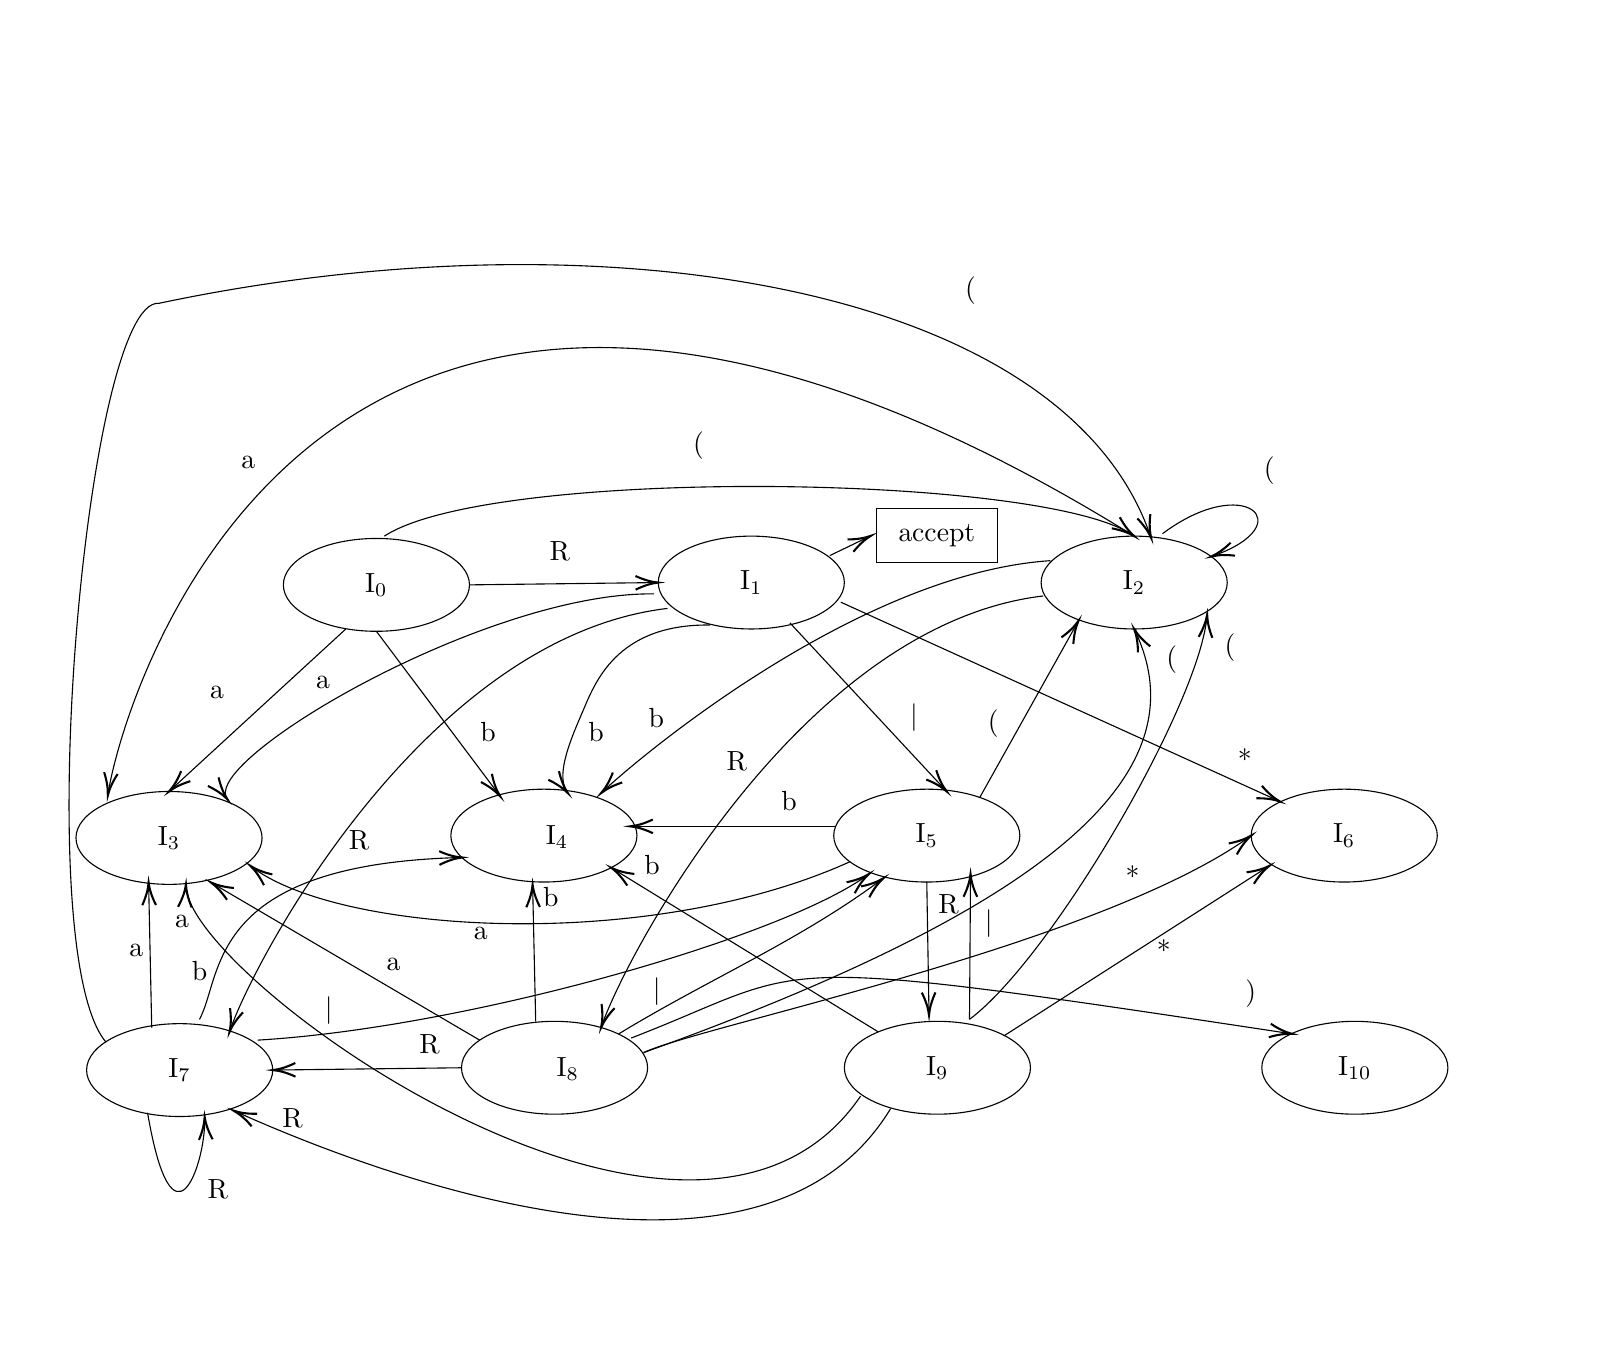
\begin{tikzpicture}[x=0.75pt,y=0.75pt,yscale=-1,xscale=1]
%uncomment if require: \path (0,505); %set diagram left start at 0, and has height of 505

%Shape: Ellipse [id:dp3219021087638878] 
\draw   (186.12,284.46) .. controls (186.12,272.1) and (206.2,262.09) .. (230.96,262.09) .. controls (255.72,262.09) and (275.79,272.1) .. (275.79,284.46) .. controls (275.79,296.81) and (255.72,306.83) .. (230.96,306.83) .. controls (206.2,306.83) and (186.12,296.81) .. (186.12,284.46) -- cycle ;
%Shape: Ellipse [id:dp5797977201007385] 
\draw   (5.5,285.58) .. controls (5.5,273.22) and (25.57,263.21) .. (50.34,263.21) .. controls (75.1,263.21) and (95.17,273.22) .. (95.17,285.58) .. controls (95.17,297.93) and (75.1,307.95) .. (50.34,307.95) .. controls (25.57,307.95) and (5.5,297.93) .. (5.5,285.58) -- cycle ;
%Shape: Ellipse [id:dp3666744957948871] 
\draw   (370.59,284.46) .. controls (370.59,272.1) and (390.66,262.09) .. (415.42,262.09) .. controls (440.18,262.09) and (460.26,272.1) .. (460.26,284.46) .. controls (460.26,296.81) and (440.18,306.83) .. (415.42,306.83) .. controls (390.66,306.83) and (370.59,296.81) .. (370.59,284.46) -- cycle ;
%Shape: Ellipse [id:dp90334119598768] 
\draw   (571.71,284.46) .. controls (571.71,272.1) and (591.78,262.09) .. (616.54,262.09) .. controls (641.3,262.09) and (661.38,272.1) .. (661.38,284.46) .. controls (661.38,296.81) and (641.3,306.83) .. (616.54,306.83) .. controls (591.78,306.83) and (571.71,296.81) .. (571.71,284.46) -- cycle ;
%Shape: Ellipse [id:dp5924602957458678] 
\draw   (286.04,162.54) .. controls (286.04,150.19) and (306.11,140.17) .. (330.88,140.17) .. controls (355.64,140.17) and (375.71,150.19) .. (375.71,162.54) .. controls (375.71,174.9) and (355.64,184.91) .. (330.88,184.91) .. controls (306.11,184.91) and (286.04,174.9) .. (286.04,162.54) -- cycle ;
%Shape: Ellipse [id:dp16247908465839256] 
\draw   (105.42,163.66) .. controls (105.42,151.3) and (125.49,141.29) .. (150.25,141.29) .. controls (175.02,141.29) and (195.09,151.3) .. (195.09,163.66) .. controls (195.09,176.01) and (175.02,186.03) .. (150.25,186.03) .. controls (125.49,186.03) and (105.42,176.01) .. (105.42,163.66) -- cycle ;
%Shape: Ellipse [id:dp8357711340177556] 
\draw   (470.51,162.54) .. controls (470.51,150.19) and (490.58,140.17) .. (515.34,140.17) .. controls (540.1,140.17) and (560.18,150.19) .. (560.18,162.54) .. controls (560.18,174.9) and (540.1,184.91) .. (515.34,184.91) .. controls (490.58,184.91) and (470.51,174.9) .. (470.51,162.54) -- cycle ;
%Shape: Ellipse [id:dp4437946742143273] 
\draw   (191.25,396.31) .. controls (191.25,383.95) and (211.32,373.94) .. (236.08,373.94) .. controls (260.84,373.94) and (280.92,383.95) .. (280.92,396.31) .. controls (280.92,408.66) and (260.84,418.68) .. (236.08,418.68) .. controls (211.32,418.68) and (191.25,408.66) .. (191.25,396.31) -- cycle ;
%Shape: Ellipse [id:dp5730777042280517] 
\draw   (10.62,397.43) .. controls (10.62,385.07) and (30.7,375.06) .. (55.46,375.06) .. controls (80.22,375.06) and (100.29,385.07) .. (100.29,397.43) .. controls (100.29,409.78) and (80.22,419.8) .. (55.46,419.8) .. controls (30.7,419.8) and (10.62,409.78) .. (10.62,397.43) -- cycle ;
%Shape: Ellipse [id:dp7459100921882429] 
\draw   (375.71,396.31) .. controls (375.71,383.95) and (395.78,373.94) .. (420.55,373.94) .. controls (445.31,373.94) and (465.38,383.95) .. (465.38,396.31) .. controls (465.38,408.66) and (445.31,418.68) .. (420.55,418.68) .. controls (395.78,418.68) and (375.71,408.66) .. (375.71,396.31) -- cycle ;
%Shape: Ellipse [id:dp5441225352938486] 
\draw   (576.83,396.31) .. controls (576.83,383.95) and (596.9,373.94) .. (621.66,373.94) .. controls (646.43,373.94) and (666.5,383.95) .. (666.5,396.31) .. controls (666.5,408.66) and (646.43,418.68) .. (621.66,418.68) .. controls (596.9,418.68) and (576.83,408.66) .. (576.83,396.31) -- cycle ;
%Straight Lines [id:da9720686438396098] 
\draw    (195.09,163.66) -- (284.04,162.56) ;
\draw [shift={(286.04,162.54)}, rotate = 539.3] [color={rgb, 255:red, 0; green, 0; blue, 0 }  ][line width=0.75]    (10.93,-3.29) .. controls (6.95,-1.4) and (3.31,-0.3) .. (0,0) .. controls (3.31,0.3) and (6.95,1.4) .. (10.93,3.29)   ;
%Curve Lines [id:da7854761753809378] 
\draw    (154.1,140.17) .. controls (204.82,106.95) and (468.36,109.91) .. (514.02,139.27) ;
\draw [shift={(515.34,140.17)}, rotate = 215.96] [color={rgb, 255:red, 0; green, 0; blue, 0 }  ][line width=0.75]    (10.93,-3.29) .. controls (6.95,-1.4) and (3.31,-0.3) .. (0,0) .. controls (3.31,0.3) and (6.95,1.4) .. (10.93,3.29)   ;
%Straight Lines [id:da3162327265476035] 
\draw    (135.52,184.91) -- (51.81,261.85) ;
\draw [shift={(50.34,263.21)}, rotate = 317.40999999999997] [color={rgb, 255:red, 0; green, 0; blue, 0 }  ][line width=0.75]    (10.93,-3.29) .. controls (6.95,-1.4) and (3.31,-0.3) .. (0,0) .. controls (3.31,0.3) and (6.95,1.4) .. (10.93,3.29)   ;
%Straight Lines [id:da009403658813172733] 
\draw    (150.25,186.03) -- (208.62,263.84) ;
\draw [shift={(209.82,265.44)}, rotate = 233.13] [color={rgb, 255:red, 0; green, 0; blue, 0 }  ][line width=0.75]    (10.93,-3.29) .. controls (6.95,-1.4) and (3.31,-0.3) .. (0,0) .. controls (3.31,0.3) and (6.95,1.4) .. (10.93,3.29)   ;
%Straight Lines [id:da25547827220686226] 
\draw    (349.5,182) -- (423.67,261.74) ;
\draw [shift={(425.03,263.21)}, rotate = 227.07] [color={rgb, 255:red, 0; green, 0; blue, 0 }  ][line width=0.75]    (10.93,-3.29) .. controls (6.95,-1.4) and (3.31,-0.3) .. (0,0) .. controls (3.31,0.3) and (6.95,1.4) .. (10.93,3.29)   ;
%Straight Lines [id:da771853946774018] 
\draw    (415.42,306.83) -- (416.47,369) ;
\draw [shift={(416.5,371)}, rotate = 269.04] [color={rgb, 255:red, 0; green, 0; blue, 0 }  ][line width=0.75]    (10.93,-3.29) .. controls (6.95,-1.4) and (3.31,-0.3) .. (0,0) .. controls (3.31,0.3) and (6.95,1.4) .. (10.93,3.29)   ;
%Straight Lines [id:da5858672387564601] 
\draw    (374,172) -- (583.68,267.17) ;
\draw [shift={(585.5,268)}, rotate = 204.41] [color={rgb, 255:red, 0; green, 0; blue, 0 }  ][line width=0.75]    (10.93,-3.29) .. controls (6.95,-1.4) and (3.31,-0.3) .. (0,0) .. controls (3.31,0.3) and (6.95,1.4) .. (10.93,3.29)   ;
%Curve Lines [id:da03884922106095501] 
\draw    (290.5,175) .. controls (174.27,188.79) and (92,343.26) .. (80,377.52) ;
\draw [shift={(79.5,379)}, rotate = 287.88] [color={rgb, 255:red, 0; green, 0; blue, 0 }  ][line width=0.75]    (10.93,-3.29) .. controls (6.95,-1.4) and (3.31,-0.3) .. (0,0) .. controls (3.31,0.3) and (6.95,1.4) .. (10.93,3.29)   ;
%Curve Lines [id:da5661969095284136] 
\draw    (471.5,169) .. controls (355.27,182.79) and (271.06,341.14) .. (259,375.52) ;
\draw [shift={(258.5,377)}, rotate = 287.88] [color={rgb, 255:red, 0; green, 0; blue, 0 }  ][line width=0.75]    (10.93,-3.29) .. controls (6.95,-1.4) and (3.31,-0.3) .. (0,0) .. controls (3.31,0.3) and (6.95,1.4) .. (10.93,3.29)   ;
%Curve Lines [id:da7355868184419707] 
\draw    (273,382) .. controls (363.5,347) and (327.5,340) .. (591.5,380) ;
\draw [shift={(591.5,380)}, rotate = 188.62] [color={rgb, 255:red, 0; green, 0; blue, 0 }  ][line width=0.75]    (10.93,-3.29) .. controls (6.95,-1.4) and (3.31,-0.3) .. (0,0) .. controls (3.31,0.3) and (6.95,1.4) .. (10.93,3.29)   ;
%Curve Lines [id:da5645087822568116] 
\draw    (284,168) .. controls (238.34,167.44) and (174.79,192.93) .. (130.28,218.62) .. controls (97.61,237.48) and (75.19,256.45) .. (77.63,265.3) ;
\draw [shift={(78.5,267)}, rotate = 231.15] [color={rgb, 255:red, 0; green, 0; blue, 0 }  ][line width=0.75]    (10.93,-3.29) .. controls (6.95,-1.4) and (3.31,-0.3) .. (0,0) .. controls (3.31,0.3) and (6.95,1.4) .. (10.93,3.29)   ;
%Curve Lines [id:da8728567793210882] 
\draw    (311,183) .. controls (265.34,182.44) and (255.28,211.62) .. (249.5,225) .. controls (244.09,237.51) and (237.1,253.8) .. (241.43,262.34) ;
\draw [shift={(242.5,264)}, rotate = 231.15] [color={rgb, 255:red, 0; green, 0; blue, 0 }  ][line width=0.75]    (10.93,-3.29) .. controls (6.95,-1.4) and (3.31,-0.3) .. (0,0) .. controls (3.31,0.3) and (6.95,1.4) .. (10.93,3.29)   ;
%Curve Lines [id:da11150423076978222] 
\draw    (529,139) .. controls (568.6,109.3) and (595.95,134.49) .. (553.8,149.55) ;
\draw [shift={(552.5,150)}, rotate = 341.18] [color={rgb, 255:red, 0; green, 0; blue, 0 }  ][line width=0.75]    (10.93,-3.29) .. controls (6.95,-1.4) and (3.31,-0.3) .. (0,0) .. controls (3.31,0.3) and (6.95,1.4) .. (10.93,3.29)   ;
%Curve Lines [id:da35067003568588295] 
\draw    (515.34,140.17) .. controls (121.48,-104.53) and (28.35,217.44) .. (21.04,263.85) ;
\draw [shift={(20.84,265.17)}, rotate = 277.83] [color={rgb, 255:red, 0; green, 0; blue, 0 }  ][line width=0.75]    (10.93,-3.29) .. controls (6.95,-1.4) and (3.31,-0.3) .. (0,0) .. controls (3.31,0.3) and (6.95,1.4) .. (10.93,3.29)   ;
%Curve Lines [id:da23538240684598] 
\draw    (475,152) .. controls (385.33,157.88) and (282.69,241.55) .. (259.8,262.78) ;
\draw [shift={(258.5,264)}, rotate = 316.47] [color={rgb, 255:red, 0; green, 0; blue, 0 }  ][line width=0.75]    (10.93,-3.29) .. controls (6.95,-1.4) and (3.31,-0.3) .. (0,0) .. controls (3.31,0.3) and (6.95,1.4) .. (10.93,3.29)   ;
%Curve Lines [id:da37523692698976685] 
\draw    (93,383) .. controls (193.49,377.06) and (344.45,333.88) .. (386.27,303.9) ;
\draw [shift={(387.5,303)}, rotate = 503.13] [color={rgb, 255:red, 0; green, 0; blue, 0 }  ][line width=0.75]    (10.93,-3.29) .. controls (6.95,-1.4) and (3.31,-0.3) .. (0,0) .. controls (3.31,0.3) and (6.95,1.4) .. (10.93,3.29)   ;
%Straight Lines [id:da8564455292691404] 
\draw    (441,266) -- (487.52,182.75) ;
\draw [shift={(488.5,181)}, rotate = 479.2] [color={rgb, 255:red, 0; green, 0; blue, 0 }  ][line width=0.75]    (10.93,-3.29) .. controls (6.95,-1.4) and (3.31,-0.3) .. (0,0) .. controls (3.31,0.3) and (6.95,1.4) .. (10.93,3.29)   ;
%Curve Lines [id:da8389145823384361] 
\draw    (378.5,297) .. controls (282.47,340.56) and (134.49,332.17) .. (90.79,299.98) ;
\draw [shift={(89.5,299)}, rotate = 398.15999999999997] [color={rgb, 255:red, 0; green, 0; blue, 0 }  ][line width=0.75]    (10.93,-3.29) .. controls (6.95,-1.4) and (3.31,-0.3) .. (0,0) .. controls (3.31,0.3) and (6.95,1.4) .. (10.93,3.29)   ;
%Straight Lines [id:da33969723496801874] 
\draw    (371,280) -- (274.5,280) ;
\draw [shift={(272.5,280)}, rotate = 360] [color={rgb, 255:red, 0; green, 0; blue, 0 }  ][line width=0.75]    (10.93,-3.29) .. controls (6.95,-1.4) and (3.31,-0.3) .. (0,0) .. controls (3.31,0.3) and (6.95,1.4) .. (10.93,3.29)   ;
%Curve Lines [id:da9985517953726066] 
\draw    (40,418) .. controls (52.13,488.81) and (67.54,442.95) .. (67.54,421.88) ;
\draw [shift={(67.5,420)}, rotate = 447.14] [color={rgb, 255:red, 0; green, 0; blue, 0 }  ][line width=0.75]    (10.93,-3.29) .. controls (6.95,-1.4) and (3.31,-0.3) .. (0,0) .. controls (3.31,0.3) and (6.95,1.4) .. (10.93,3.29)   ;
%Curve Lines [id:da5393037373239191] 
\draw    (20,384) .. controls (-17.5,340) and (10.5,25) .. (45.5,28) ;
%Curve Lines [id:da7722532448096251] 
\draw    (45.5,28) .. controls (257.44,-16.78) and (480.26,18.64) .. (522.87,139.18) ;
\draw [shift={(523.5,141)}, rotate = 251.42000000000002] [color={rgb, 255:red, 0; green, 0; blue, 0 }  ][line width=0.75]    (10.93,-3.29) .. controls (6.95,-1.4) and (3.31,-0.3) .. (0,0) .. controls (3.31,0.3) and (6.95,1.4) .. (10.93,3.29)   ;
%Straight Lines [id:da1930704542407602] 
\draw    (42,377) -- (40.54,309) ;
\draw [shift={(40.5,307)}, rotate = 448.77] [color={rgb, 255:red, 0; green, 0; blue, 0 }  ][line width=0.75]    (10.93,-3.29) .. controls (6.95,-1.4) and (3.31,-0.3) .. (0,0) .. controls (3.31,0.3) and (6.95,1.4) .. (10.93,3.29)   ;
%Curve Lines [id:da8884229271696089] 
\draw    (65,373) .. controls (76.44,352.1) and (67.59,298.54) .. (189.65,295.05) ;
\draw [shift={(191.5,295)}, rotate = 538.61] [color={rgb, 255:red, 0; green, 0; blue, 0 }  ][line width=0.75]    (10.93,-3.29) .. controls (6.95,-1.4) and (3.31,-0.3) .. (0,0) .. controls (3.31,0.3) and (6.95,1.4) .. (10.93,3.29)   ;
%Curve Lines [id:da13055573215355598] 
\draw    (267,380) .. controls (309.08,354.26) and (353.6,335.38) .. (393.3,305.9) ;
\draw [shift={(394.5,305)}, rotate = 503.13] [color={rgb, 255:red, 0; green, 0; blue, 0 }  ][line width=0.75]    (10.93,-3.29) .. controls (6.95,-1.4) and (3.31,-0.3) .. (0,0) .. controls (3.31,0.3) and (6.95,1.4) .. (10.93,3.29)   ;
%Straight Lines [id:da5564516670181785] 
\draw    (191.25,396.31) -- (102.29,397.4) ;
\draw [shift={(100.29,397.43)}, rotate = 359.3] [color={rgb, 255:red, 0; green, 0; blue, 0 }  ][line width=0.75]    (10.93,-3.29) .. controls (6.95,-1.4) and (3.31,-0.3) .. (0,0) .. controls (3.31,0.3) and (6.95,1.4) .. (10.93,3.29)   ;
%Curve Lines [id:da09276489882545103] 
\draw    (279,389) .. controls (306.36,376.07) and (497.57,337.39) .. (570.61,285.24) ;
\draw [shift={(571.71,284.46)}, rotate = 503.96] [color={rgb, 255:red, 0; green, 0; blue, 0 }  ][line width=0.75]    (10.93,-3.29) .. controls (6.95,-1.4) and (3.31,-0.3) .. (0,0) .. controls (3.31,0.3) and (6.95,1.4) .. (10.93,3.29)   ;
%Curve Lines [id:da5425101005887105] 
\draw    (279,389) .. controls (472.53,319.35) and (548.74,255.64) .. (515.85,185.96) ;
\draw [shift={(515.34,184.91)}, rotate = 424.02] [color={rgb, 255:red, 0; green, 0; blue, 0 }  ][line width=0.75]    (10.93,-3.29) .. controls (6.95,-1.4) and (3.31,-0.3) .. (0,0) .. controls (3.31,0.3) and (6.95,1.4) .. (10.93,3.29)   ;
%Straight Lines [id:da882081304982782] 
\draw    (200,383) -- (72.22,308.01) ;
\draw [shift={(70.5,307)}, rotate = 390.40999999999997] [color={rgb, 255:red, 0; green, 0; blue, 0 }  ][line width=0.75]    (10.93,-3.29) .. controls (6.95,-1.4) and (3.31,-0.3) .. (0,0) .. controls (3.31,0.3) and (6.95,1.4) .. (10.93,3.29)   ;
%Straight Lines [id:da1725844151186562] 
\draw    (227,374) -- (225.55,310) ;
\draw [shift={(225.5,308)}, rotate = 448.7] [color={rgb, 255:red, 0; green, 0; blue, 0 }  ][line width=0.75]    (10.93,-3.29) .. controls (6.95,-1.4) and (3.31,-0.3) .. (0,0) .. controls (3.31,0.3) and (6.95,1.4) .. (10.93,3.29)   ;
%Straight Lines [id:da42871673894639795] 
\draw    (392,379) -- (265.2,301.05) ;
\draw [shift={(263.5,300)}, rotate = 391.58000000000004] [color={rgb, 255:red, 0; green, 0; blue, 0 }  ][line width=0.75]    (10.93,-3.29) .. controls (6.95,-1.4) and (3.31,-0.3) .. (0,0) .. controls (3.31,0.3) and (6.95,1.4) .. (10.93,3.29)   ;
%Curve Lines [id:da8407552386217021] 
\draw    (383.5,410) .. controls (303.31,527.81) and (61.4,354.53) .. (58.51,309.33) ;
\draw [shift={(58.5,308)}, rotate = 452.66] [color={rgb, 255:red, 0; green, 0; blue, 0 }  ][line width=0.75]    (10.93,-3.29) .. controls (6.95,-1.4) and (3.31,-0.3) .. (0,0) .. controls (3.31,0.3) and (6.95,1.4) .. (10.93,3.29)   ;
%Curve Lines [id:da04457491957875015] 
\draw    (436,373) .. controls (475.4,343.45) and (545.36,223.67) .. (550.32,179.94) ;
\draw [shift={(550.5,178)}, rotate = 454.09] [color={rgb, 255:red, 0; green, 0; blue, 0 }  ][line width=0.75]    (10.93,-3.29) .. controls (6.95,-1.4) and (3.31,-0.3) .. (0,0) .. controls (3.31,0.3) and (6.95,1.4) .. (10.93,3.29)   ;
%Straight Lines [id:da6383474074976259] 
\draw    (452.5,381) -- (578.82,300.08) ;
\draw [shift={(580.5,299)}, rotate = 507.36] [color={rgb, 255:red, 0; green, 0; blue, 0 }  ][line width=0.75]    (10.93,-3.29) .. controls (6.95,-1.4) and (3.31,-0.3) .. (0,0) .. controls (3.31,0.3) and (6.95,1.4) .. (10.93,3.29)   ;
%Curve Lines [id:da7126329870392456] 
\draw    (398,416) .. controls (333.16,522.92) and (134.53,440.68) .. (83.02,417.68) ;
\draw [shift={(81.5,417)}, rotate = 384.18] [color={rgb, 255:red, 0; green, 0; blue, 0 }  ][line width=0.75]    (10.93,-3.29) .. controls (6.95,-1.4) and (3.31,-0.3) .. (0,0) .. controls (3.31,0.3) and (6.95,1.4) .. (10.93,3.29)   ;
%Straight Lines [id:da013535075432713706] 
\draw    (436,373) -- (436.49,305) ;
\draw [shift={(436.5,303)}, rotate = 450.41] [color={rgb, 255:red, 0; green, 0; blue, 0 }  ][line width=0.75]    (10.93,-3.29) .. controls (6.95,-1.4) and (3.31,-0.3) .. (0,0) .. controls (3.31,0.3) and (6.95,1.4) .. (10.93,3.29)   ;
%Shape: Rectangle [id:dp6819443275458348] 
\draw   (391,127) -- (449.5,127) -- (449.5,153) -- (391,153) -- cycle ;
%Straight Lines [id:da9536906744074418] 
\draw    (368.71,149.54) -- (386.7,140.87) ;
\draw [shift={(388.5,140)}, rotate = 514.26] [color={rgb, 255:red, 0; green, 0; blue, 0 }  ][line width=0.75]    (10.93,-3.29) .. controls (6.95,-1.4) and (3.31,-0.3) .. (0,0) .. controls (3.31,0.3) and (6.95,1.4) .. (10.93,3.29)   ;

% Text Node
\draw (721,21) node    {};
% Text Node
\draw (701,71) node    {};
% Text Node
\draw (722,251) node    {};
% Text Node
\draw (702,301) node    {};
% Text Node
\draw (150.25,163.66) node   [align=left] {I\textsubscript{0}};
% Text Node
\draw (515.34,162.54) node   [align=left] {I\textsubscript{2}};
% Text Node
\draw (330.88,162.54) node   [align=left] {I\textsubscript{1}};
% Text Node
\draw (415.42,284.46) node   [align=left] {I\textsubscript{5}};
% Text Node
\draw (237.36,285.02) node   [align=left] {I\textsubscript{4}};
% Text Node
\draw (50.34,285.58) node   [align=left] {I\textsubscript{3}};
% Text Node
\draw (616.54,284.46) node   [align=left] {I\textsubscript{6}};
% Text Node
\draw (420.55,396.31) node   [align=left] {I\textsubscript{9}};
% Text Node
\draw (242.49,396.87) node   [align=left] {I\textsubscript{8}};
% Text Node
\draw (55.46,397.43) node   [align=left] {I\textsubscript{7}};
% Text Node
\draw (621.66,396.31) node   [align=left] {I\textsubscript{10}};
% Text Node
\draw (238.64,147.44) node   [align=left] {R};
% Text Node
\draw (305.47,96.7) node   [align=left] {(};
% Text Node
\draw (568.59,247.84) node   [align=left] {*};
% Text Node
\draw (204.06,234.68) node   [align=left] {b};
% Text Node
\draw (409.26,227.68) node   [align=left] {$|$};
% Text Node
\draw (141.86,286.7) node   [align=left] {R};
% Text Node
\draw (73.39,215.67) node   [align=left] {a};
% Text Node
\draw (323.86,248.7) node   [align=left] {R};
% Text Node
\draw (425.86,317.5) node   [align=left] {R};
% Text Node
\draw (571.47,360.5) node   [align=left] {)};
% Text Node
\draw (124.39,210.67) node   [align=left] {a};
% Text Node
\draw (256.06,234.68) node   [align=left] {b};
% Text Node
\draw (580.47,108.7) node   [align=left] {(};
% Text Node
\draw (88.39,104.67) node   [align=left] {a};
% Text Node
\draw (285.06,227.68) node   [align=left] {b};
% Text Node
\draw (447.47,230.7) node   [align=left] {(};
% Text Node
\draw (200.39,331.67) node   [align=left] {a};
% Text Node
\draw (349.06,267.5) node   [align=left] {b};
% Text Node
\draw (127.26,368.68) node   [align=left] {$|$};
% Text Node
\draw (73.86,454.7) node   [align=left] {R};
% Text Node
\draw (436.47,21.7) node   [align=left] {(};
% Text Node
\draw (34.39,339.67) node   [align=left] {a};
% Text Node
\draw (65,349.68) node   [align=left] {b};
% Text Node
\draw (285.26,359.68) node   [align=left] {$|$};
% Text Node
\draw (175.86,384.7) node   [align=left] {R};
% Text Node
\draw (514.59,303.84) node   [align=left] {*};
% Text Node
\draw (533.47,199.7) node   [align=left] {(};
% Text Node
\draw (158.39,346.67) node   [align=left] {a};
% Text Node
\draw (234.25,314) node   [align=left] {b};
% Text Node
\draw (283.06,298.5) node   [align=left] {b};
% Text Node
\draw (56.5,325.67) node   [align=left] {a};
% Text Node
\draw (561.47,193.7) node   [align=left] {(};
% Text Node
\draw (529.59,339.84) node   [align=left] {*};
% Text Node
\draw (109.86,420.7) node   [align=left] {R};
% Text Node
\draw (445.26,326.68) node   [align=left] {$|$};
% Text Node
\draw (420.25,140) node   [align=left] {accept};


\end{tikzpicture}



    \caption{SLR Parsing table}
    \label{fig:my_label}
\end{figure}
\begin{table}[H]
\centering
\begin{tabular}{|l|l|l|l|l|l|l|l|l|l|}
\hline
\multirow{\textbf{STATE}} & \multicolumn{7}{l|}{\textbf{ACTION}}    
& \multicolumn{2}{l|}{\textbf{GOTO}} \\ \cline{2-10} 
                                & $|$                                               & *                                               & (                                               & )   & a                                               & b                                               & \$     & S                & R               \\ \hline
\textbf{0}                      &                                                 &                                                 &                                s2                 &     & s3                                              & s4                                              &        &                  & 1               \\ \hline
\textbf{1}                      & s5                                              & s6                                              & s2                                              &     & s3                                              & s4                                              & accept &                  & 7               \\ \hline
\textbf{2}                      &                                                 &                                                 & s2                                              &     & s3                                              & s4                                              &        &                  & 8               \\ \hline
\textbf{3}                      & r6                                              & r6                                              & r6                                              & r6  & r6                                              & r6                                              & r6     &                  &                 \\ \hline
\textbf{4}                      & r7                                              & r7                                              & r7                                              & r7  & r7                                              & r7                                              & r7     &                  &                 \\ \hline
\textbf{5}                      &                                                 &                                                 & s2                                              &     & s3                                              & s4                                              &        &                  & 9               \\ \hline
\textbf{6}                      & r4                                              & r4                                              & r4                                              & r4  & r4                                              & r4                                              & r4     &                  &                 \\ \hline
\textbf{7}                      & \begin{tabular}[c]{@{}l@{}}r3\\ s5\end{tabular} & \begin{tabular}[c]{@{}l@{}}r3\\ s6\end{tabular} & \begin{tabular}[c]{@{}l@{}}r3\\ s2\end{tabular} & r3  & \begin{tabular}[c]{@{}l@{}}r3\\ s3\end{tabular} & \begin{tabular}[c]{@{}l@{}}r3\\ s4\end{tabular} & r3     &                  & 7               \\ \hline
\textbf{8}                      & s5                                              & s6                                              &                             s2                    & s10 &                                         s3        &                     s4                            &        &                  & 7               \\ \hline
\textbf{9}                      & \begin{tabular}[c]{@{}l@{}}r2\\ s5\end{tabular} & \begin{tabular}[c]{@{}l@{}}r2\\ s6\end{tabular} & \begin{tabular}[c]{@{}l@{}}r2\\ s2\end{tabular} & r2  & \begin{tabular}[c]{@{}l@{}}r2\\ s3\end{tabular} & \begin{tabular}[c]{@{}l@{}}r2\\ s4\end{tabular} & r2     &                  & 7               \\ \hline
\textbf{10}                     & r5                                              & r5                                              & r5                                              & r5  & r5                                              & r5                                              & r5     &                  &                 \\ \hline
\end{tabular}
\caption{Parse table for SLR(1) before disambiguation}
\end{table}
As we can see, there are 4 shift reduce conflicts. These arise due to undefined precedence and associativity of $|$ , concatenation and $*$. To solve the conflicts, we follow the following disambiguation rules - 
\begin{enumerate}
    \item \textbf{Precedence of * $>$ precedence of concatenation $>$ precedence of $|$}
    \item \textbf{$|$ and concatenation are left associative}
\end{enumerate}
\textbf{The following steps are taken to disambiguate - }
\begin{itemize}
    \item \textbf{Row 7 Terminal $|$ :} Precedence of concatenation  $>$ Precedence of $|$ hence r3
    \item \textbf{Row 7 Terminal $*$ :} Precedence of $*$  $>$ Precedence of concatenation hence s6
    \item \textbf{Row 7 Terminal $($ :} concatenation is left associative hence r3
    \item \textbf{Row 7 Terminal $a$ :} concatenation is left associative hence r3
    \item \textbf{Row 7 Terminal $b$ :} concatenation is left associative hence r3
    \item \textbf{Row 9 Terminal $|$ :} $|$ is left associative hence r2
    \item \textbf{Row 9 Terminal $*$ :} Precedence of $*$  $>$ Precedence of $|$ hence s6
    \item \textbf{Row 9 Terminal $($ :} Precedence of concatenation  $>$ Precedence of $|$ hence s2
    \item \textbf{Row 9 Terminal $a$ :} Precedence of concatenation  $>$ Precedence of $|$ hence s3
    \item \textbf{Row 9 Terminal $b$ :} Precedence of concatenation  $>$ Precedence of $|$ hence s4
\end{itemize}
\textbf{After disambiguation}

 \begin{table}[H]
 \centering
\begin{tabular}{|l|l|l|l|l|l|l|l|l|l|}
\hline
\multirow{\textbf{STATE}} & \multicolumn{7}{l|}{\textbf{ACTION}} & \multicolumn{2}{l|}{\textbf{GOTO}} \\ \cline{2-10} 
            & $|$  & *  & (  & )   & a  & b  & \$     & S & R \\ \hline
\textbf{0}  &    &    &    &     & s3 & s4 &        &   & 1 \\ \hline
\textbf{1}  & s5 & s6 & s2 &     & s3 & s4 & accept &   & 7 \\ \hline
\textbf{2}  &    &    & s2 &     & s3 & s4 &        &   & 8 \\ \hline
\textbf{3}  & r6 & r6 & r6 & r6  & r6 & r6 & r6     &   &   \\ \hline
\textbf{4}  & r7 & r7 & r7 & r7  & r7 & r7 & r7     &   &   \\ \hline
\textbf{5}  &    &    & s2 &     & s3 & s4 &        &   & 9 \\ \hline
\textbf{6}  & r4 & r4 & r4 & r4  & r4 & r4 & r4     &   &   \\ \hline
\textbf{7}  & r3 & s6 & r3 & r3  & r3 & r3 & r3     &   & 7 \\ \hline
\textbf{8}  & s5 & s6 &   s2 & s10 & s3    & s4 &        &   & 7 \\ \hline
\textbf{9}  & r2 & s6 & s2 & r2  & s3 & s4 & r2     &   & 7 \\ \hline
\textbf{10} & r5 & r5 & r5 & r5  & r5 & r5 & r5     &   &   \\ \hline
\end{tabular}
\caption{Parse table for SLR(1) after disambiguation}

\end{table}
\section*{Question}
\question{\textbf{Dissertation Parser}}\\~\\
\textbf{Tools used :}
\begin{itemize}
    \item flex 2.6.4
    \item bison (GNU Bison) 3.0.4
    \item g++ 7.4.0
\end{itemize}
To run the parser, run the following program :

\begin{cplusplus}
bash run.sh <INPUT_FILE>
\end{cplusplus}
\textbf{Example}:
\begin{cplusplus}
bash run.sh samplethesis.txt
\end{cplusplus}

The output shows in \textbf{STDOUT}\\
The errors will be redirected to \textbf{STDERR}.
\end{questions}
\end{document}


 